\begin{figure}[ht]
\begin{center}
\begin{adjustbox}{width=0.5\textwidth}

    \tikzset{every picture/.style={line width=0.75pt}} %set default line width to 0.75pt        
    
    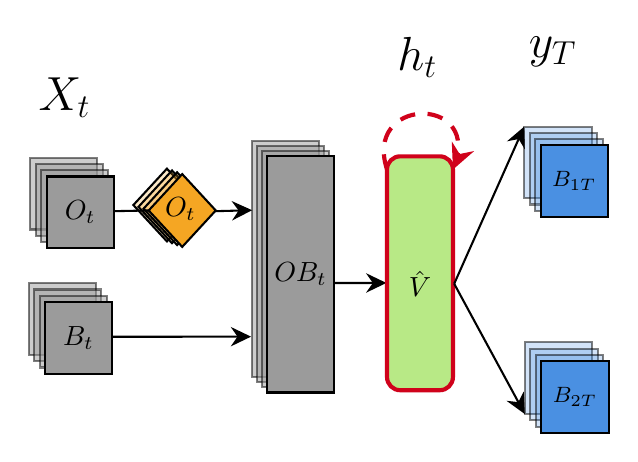
\begin{tikzpicture}[x=0.75pt,y=0.75pt,yscale=-1,xscale=1]
    %uncomment if require: \path (0,300); %set diagram left start at 0, and has height of 300
    
    %Shape: Diamond [id:dp06877884521197963] 
    \draw  [fill={rgb, 255:red, 245; green, 166; blue, 35 }  ,fill opacity=0.25 ] (263.6,117.28) -- (279.77,134.81) -- (263.6,152.33) -- (247.43,134.81) -- cycle ;
    %Shape: Diamond [id:dp5019197402707816] 
    \draw  [fill={rgb, 255:red, 245; green, 166; blue, 35 }  ,fill opacity=0.25 ] (266.05,118.16) -- (282.22,135.68) -- (266.05,153.2) -- (249.89,135.68) -- cycle ;
    %Shape: Diamond [id:dp6628494024847519] 
    \draw  [fill={rgb, 255:red, 245; green, 166; blue, 35 }  ,fill opacity=0.25 ] (268.51,119.04) -- (284.68,136.56) -- (268.51,154.08) -- (252.34,136.56) -- cycle ;
    %Shape: Rectangle [id:dp8304682723722553] 
    \draw  [color={rgb, 255:red, 0; green, 0; blue, 0 }  ,draw opacity=0.5 ][fill={rgb, 255:red, 155; green, 155; blue, 155 }  ,fill opacity=0.5 ] (304.41,104.01) -- (336.92,104.01) -- (336.92,217.74) -- (304.41,217.74) -- cycle ;
    %Shape: Rectangle [id:dp33657106031779216] 
    \draw  [color={rgb, 255:red, 0; green, 0; blue, 0 }  ,draw opacity=0.5 ][fill={rgb, 255:red, 155; green, 155; blue, 155 }  ,fill opacity=0.5 ] (306.86,106.47) -- (339.38,106.47) -- (339.38,220.2) -- (306.86,220.2) -- cycle ;
    %Shape: Rectangle [id:dp6698304713342962] 
    \draw  [color={rgb, 255:red, 0; green, 0; blue, 0 }  ,draw opacity=0.5 ][fill={rgb, 255:red, 155; green, 155; blue, 155 }  ,fill opacity=0.5 ] (309.32,108.93) -- (341.84,108.93) -- (341.84,222.66) -- (309.32,222.66) -- cycle ;
    %Shape: Diamond [id:dp7704333366065277] 
    \draw  [fill={rgb, 255:red, 245; green, 166; blue, 35 }  ,fill opacity=1 ] (270.97,119.91) -- (287.13,137.43) -- (270.97,154.96) -- (254.8,137.43) -- cycle ;
    %Straight Lines [id:da34159449213041837] 
    \draw    (286.94,137.77) -- (301.65,137.38) ;
    \draw [shift={(304.65,137.3)}, rotate = 178.49] [fill={rgb, 255:red, 0; green, 0; blue, 0 }  ][line width=0.08]  [draw opacity=0] (9.82,-4.72) -- (0,0) -- (9.82,4.72) -- (6.52,0) -- cycle    ;
    %Straight Lines [id:da8208338090000002] 
    \draw [fill={rgb, 255:red, 155; green, 155; blue, 155 }  ,fill opacity=1 ]   (215.09,198.3) -- (301.13,198.22) ;
    \draw [shift={(304.13,198.22)}, rotate = 179.95] [fill={rgb, 255:red, 0; green, 0; blue, 0 }  ][line width=0.08]  [draw opacity=0] (9.82,-4.72) -- (0,0) -- (9.82,4.72) -- (6.52,0) -- cycle    ;
    %Straight Lines [id:da7791621502079311] 
    \draw [fill={rgb, 255:red, 155; green, 155; blue, 155 }  ,fill opacity=1 ]   (336.42,172.36) -- (366.33,172.35) ;
    \draw [shift={(369.33,172.35)}, rotate = 179.97] [fill={rgb, 255:red, 0; green, 0; blue, 0 }  ][line width=0.08]  [draw opacity=0] (9.82,-4.72) -- (0,0) -- (9.82,4.72) -- (6.52,0) -- cycle    ;
    %Shape: Rectangle [id:dp3847312278870677] 
    \draw  [color={rgb, 255:red, 0; green, 0; blue, 0 }  ,draw opacity=0.5 ][fill={rgb, 255:red, 155; green, 155; blue, 155 }  ,fill opacity=0.5 ] (197.01,172.53) -- (229.26,172.53) -- (229.26,207.05) -- (197.01,207.05) -- cycle ;
    %Shape: Rectangle [id:dp5169374919332619] 
    \draw  [color={rgb, 255:red, 0; green, 0; blue, 0 }  ,draw opacity=0.5 ][fill={rgb, 255:red, 155; green, 155; blue, 155 }  ,fill opacity=0.5 ] (199.63,175.51) -- (231.88,175.51) -- (231.88,210.03) -- (199.63,210.03) -- cycle ;
    %Shape: Rectangle [id:dp7025889851900418] 
    \draw  [color={rgb, 255:red, 0; green, 0; blue, 0 }  ,draw opacity=0.5 ][fill={rgb, 255:red, 155; green, 155; blue, 155 }  ,fill opacity=0.5 ] (202.27,178.56) -- (234.53,178.56) -- (234.53,213.08) -- (202.27,213.08) -- cycle ;
    %Shape: Rectangle [id:dp34989838660273853] 
    \draw  [fill={rgb, 255:red, 155; green, 155; blue, 155 }  ,fill opacity=1 ] (204.86,181.5) -- (237.11,181.5) -- (237.11,216.02) -- (204.86,216.02) -- cycle ;
    %Shape: Rectangle [id:dp10413248734443492] 
    \draw  [fill={rgb, 255:red, 155; green, 155; blue, 155 }  ,fill opacity=1 ] (311.77,111.39) -- (344.29,111.39) -- (344.29,225.12) -- (311.77,225.12) -- cycle ;
    %Shape: Rectangle [id:dp5251277777045114] 
    \draw  [color={rgb, 255:red, 0; green, 0; blue, 0 }  ,draw opacity=0.5 ][fill={rgb, 255:red, 155; green, 155; blue, 155 }  ,fill opacity=0.5 ] (197.83,112.08) -- (230.08,112.08) -- (230.08,146.6) -- (197.83,146.6) -- cycle ;
    %Shape: Rectangle [id:dp04395321919357453] 
    \draw  [color={rgb, 255:red, 0; green, 0; blue, 0 }  ,draw opacity=0.5 ][fill={rgb, 255:red, 155; green, 155; blue, 155 }  ,fill opacity=0.5 ] (200.45,115.06) -- (232.7,115.06) -- (232.7,149.58) -- (200.45,149.58) -- cycle ;
    %Shape: Rectangle [id:dp5987068943888822] 
    \draw  [color={rgb, 255:red, 0; green, 0; blue, 0 }  ,draw opacity=0.5 ][fill={rgb, 255:red, 155; green, 155; blue, 155 }  ,fill opacity=0.5 ] (203.09,118.11) -- (235.35,118.11) -- (235.35,152.63) -- (203.09,152.63) -- cycle ;
    %Shape: Rectangle [id:dp34752966033388544] 
    \draw  [fill={rgb, 255:red, 155; green, 155; blue, 155 }  ,fill opacity=1 ] (205.68,121.05) -- (237.93,121.05) -- (237.93,155.57) -- (205.68,155.57) -- cycle ;
    %Straight Lines [id:da167964927096784] 
    \draw    (237.82,137.77) -- (254.8,137.43) ;
    %Rounded Rect [id:dp23035038317630208] 
    \draw  [color={rgb, 255:red, 208; green, 2; blue, 27 }  ,draw opacity=1 ][fill={rgb, 255:red, 184; green, 233; blue, 134 }  ,fill opacity=1 ][line width=1.5]  (369.64,117.69) .. controls (369.64,114.18) and (372.48,111.34) .. (375.99,111.34) -- (395.05,111.34) .. controls (398.56,111.34) and (401.4,114.18) .. (401.4,117.69) -- (401.4,217.68) .. controls (401.4,221.19) and (398.56,224.03) .. (395.05,224.03) -- (375.99,224.03) .. controls (372.48,224.03) and (369.64,221.19) .. (369.64,217.68) -- cycle ;
    %Curve Lines [id:da1309582955199332] 
    \draw [color={rgb, 255:red, 208; green, 2; blue, 27 }  ,draw opacity=1 ][line width=1.5]  [dash pattern={on 5.63pt off 4.5pt}]  (369.64,117.69) .. controls (358.28,83.07) and (412.82,81.85) .. (402.76,114.05) ;
    \draw [shift={(401.4,117.69)}, rotate = 293.32] [fill={rgb, 255:red, 208; green, 2; blue, 27 }  ,fill opacity=1 ][line width=0.08]  [draw opacity=0] (12.23,-5.88) -- (0,0) -- (12.23,5.88) -- (8.12,0) -- cycle    ;
    %Shape: Rectangle [id:dp8222204045246226] 
    \draw  [color={rgb, 255:red, 0; green, 0; blue, 0 }  ,draw opacity=0.5 ][fill={rgb, 255:red, 74; green, 144; blue, 226 }  ,fill opacity=0.25 ] (435.7,97.06) -- (468.2,97.06) -- (468.2,131.57) -- (435.7,131.57) -- cycle ;
    %Shape: Rectangle [id:dp5039823026088135] 
    \draw  [color={rgb, 255:red, 0; green, 0; blue, 0 }  ,draw opacity=0.5 ][fill={rgb, 255:red, 74; green, 144; blue, 226 }  ,fill opacity=0.25 ] (438.34,100.04) -- (470.84,100.04) -- (470.84,134.54) -- (438.34,134.54) -- cycle ;
    %Shape: Rectangle [id:dp021668374233558163] 
    \draw  [color={rgb, 255:red, 0; green, 0; blue, 0 }  ,draw opacity=0.5 ][fill={rgb, 255:red, 74; green, 144; blue, 226 }  ,fill opacity=0.25 ] (441,103.09) -- (473.51,103.09) -- (473.51,137.6) -- (441,137.6) -- cycle ;
    %Shape: Rectangle [id:dp505523013710797] 
    \draw  [fill={rgb, 255:red, 74; green, 144; blue, 226 }  ,fill opacity=1 ] (443.61,106.03) -- (476.11,106.03) -- (476.11,140.53) -- (443.61,140.53) -- cycle ;
    %Shape: Rectangle [id:dp0946025609940615] 
    \draw  [color={rgb, 255:red, 0; green, 0; blue, 0 }  ,draw opacity=0.5 ][fill={rgb, 255:red, 74; green, 144; blue, 226 }  ,fill opacity=0.25 ] (436.03,200.99) -- (468.53,200.99) -- (468.53,235.5) -- (436.03,235.5) -- cycle ;
    %Shape: Rectangle [id:dp07647490089995623] 
    \draw  [color={rgb, 255:red, 0; green, 0; blue, 0 }  ,draw opacity=0.5 ][fill={rgb, 255:red, 74; green, 144; blue, 226 }  ,fill opacity=0.25 ] (438.67,203.97) -- (471.17,203.97) -- (471.17,238.47) -- (438.67,238.47) -- cycle ;
    %Shape: Rectangle [id:dp2801868133972626] 
    \draw  [color={rgb, 255:red, 0; green, 0; blue, 0 }  ,draw opacity=0.5 ][fill={rgb, 255:red, 74; green, 144; blue, 226 }  ,fill opacity=0.25 ] (441.33,207.02) -- (473.84,207.02) -- (473.84,241.53) -- (441.33,241.53) -- cycle ;
    %Shape: Rectangle [id:dp241922601816576] 
    \draw  [fill={rgb, 255:red, 74; green, 144; blue, 226 }  ,fill opacity=1 ] (443.94,209.96) -- (476.44,209.96) -- (476.44,244.46) -- (443.94,244.46) -- cycle ;
    %Straight Lines [id:da6479510532261308] 
    \draw    (402,172.73) -- (434.48,99.8) ;
    \draw [shift={(435.7,97.06)}, rotate = 114] [fill={rgb, 255:red, 0; green, 0; blue, 0 }  ][line width=0.08]  [draw opacity=0] (9.82,-4.72) -- (0,0) -- (9.82,4.72) -- (6.52,0) -- cycle    ;
    %Straight Lines [id:da5488291959914686] 
    \draw    (402,172.73) -- (434.6,232.86) ;
    \draw [shift={(436.03,235.5)}, rotate = 241.54] [fill={rgb, 255:red, 0; green, 0; blue, 0 }  ][line width=0.08]  [draw opacity=0] (9.82,-4.72) -- (0,0) -- (9.82,4.72) -- (6.52,0) -- cycle    ;
    
    % Text Node
    \draw (220.99,198.76) node  [font=\normalsize]  {$B_{t}$};
    % Text Node
    \draw (385.52,172.8) node  [font=\normalsize]  {$\hat{V}$};
    % Text Node
    \draw (270.15,136.56) node  [font=\normalsize]  {$O_{t}$};
    % Text Node
    \draw (214.34,83.25) node  [font=\LARGE]  {$X_{t}$};
    % Text Node
    \draw (328.03,168.25) node  [font=\normalsize]  {$OB_{t}$};
    % Text Node
    \draw (221.81,138.31) node  [font=\normalsize]  {$O_{t}$};
    % Text Node
    \draw (384.34,63.6) node  [font=\LARGE]  {$h_{t}$};
    % Text Node
    \draw (459.86,123.28) node  [font=\footnotesize]  {$B_{1T}$};
    % Text Node
    \draw (460.19,227.21) node  [font=\footnotesize]  {$B_{2T}$};
    % Text Node
    \draw (449.54,61) node  [font=\LARGE]  {$y_{T}$};
    
    \end{tikzpicture}

\end{adjustbox}
\end{center}
\caption{\textbf{Bifurcating Model (BM) Architecture.} The first section learns an embedding for each game context and fuses it, via concatenation, with the feature set. The embedding allows the model to learn a rich multi-dimensional representation of the game context projecting similar games into closer points in the latent space. The second section takes these fused representation over time and models them temporally using an LSTM. The LSTM is particularly suitable because it can handle time series of different lengths and explicitly model temporal dependencies. We thought to use this part of the model for extracting a high level representation of the player state which could be used for predicting measures of future disengagement and sustained engagement. Inspired by the results of \textit{Experiment 1}, this is achieved by 'branching' two shallow NNs tasked to perform churn probability and survival time estimation.}
\label{fig: rnn_1}
\end{figure}